\documentclass{report}
\usepackage[francais]{babel}
\usepackage{graphicx}
\usepackage{lmodern}
\usepackage{minted}


\begin{document}
\begin{titlepage}
  \centering
  {\scshape Institut Saint Jean Berchmans - Sainte Marie\par\vspace{0.2cm} Section informatique\par \vspace{0.2cm}}
  \vspace{1cm}
  
\includegraphics[width=0.25\textwidth]{img/image2}\par\vspace{1cm}
  {\scshape \LARGE Programmation \par}
  \vspace{0.2cm}
	{\scshape \Large The Shell Adventure\par}
  \vspace{3cm}
  {\Large\itshape Travail de fin d'étude \par réalisé par \par Jordan Dalcq \par}
  \vfill
  \scshape Année académique 2018 - 2019
  \title{The Shell Adventure}
  \author{Jordan Dalcq}
  \date{2018 - 2019}
\end{titlepage}

\tableofcontents

\pagestyle{empty}

\part*{Remerciments}

Je tiens tout d'abord à remercier mon grand père Yvan, qui m'a introduit au monde de l'informatique dés mon plus jeune âge, et de m'avoir montré aussi les joies de Linux dés mes 7 ans.
\newline
\par Je remercie mes parents Fabienne et Marc pour avoir investis en moi afin de me permettre de continuer sur ma voie vers un métier qui me pasionne.
\newline
\par Je remercie Alex Roşca, d'avoir été mon premier amis, dans cette grande aventure, merci de m'avoir permis de découvrire la programmation
\newline
\par Je remercie Monsieur David Carrera pour avoir été le seule professeur qui a été capable à me poussé au meillieur dans ma passion.
\newline
\par Je tiens aussi à remercier toutes les personne que j'ai rencontré à l'Institut Saint Jean Berchmans, pour m'avoir influencé dans ce projet d'une manière ou d'une autre.

\part{Introductions}

\section*{Contexte}
Durant quelques années j’ai été mentor au Coderdojo de Liège durant 2 ans. J’animais un atelier Python / Linux auprès de jeunes âgés entre 14 et 18 ans. Le problème lors de l’apprentissage était qu’ils ne savaient pas quelle commande / fonction utiliser dans un cas précis. Dans ce projet, j’ai décidé de me focaliser sur le terminal bash et de présenter un outil d’ apprentissage basé sur le visuel.
\chapter{Présentation}
\section{Fonctionnement}
L’idée de base est assez simple, il faut taper des commandes pour interagir avec le monde qui nous entoure.
\newline
\newline
Comme par exemple:

\begin {itemize}
  \item cd  : Pour se déplacer d’une pièce à une autre
  touch : Pour créer un objet ou bien faire apparaître une personne
  \item cp : Pour cloner un objet ou personnage
  \item mv : Pour déplacer un objet ou personnage
  \item cat : Pour connaître le contenu d’un objet ou alors l'identité d’un personnage
  \item rm : Pour jeter un objet ou “éliminer” un personnage
  \item tree : Scanner à rayon X pour voir à travers les murs
\end {itemize}

A cause du temps assez limité, j'ai implimenté un langage de programmation afin de laisser une liberté de choisir le pouvoir de chaque commande à l'utilisateur

\section{Élement}
Énumérez et décrivez, dans l’ordre et en français, les différentes parties de votre application. Il s’agit de présenter les différents éléments (ainsi que leurs caractéristiques) qui sont amenés à interagir au sein de votre programme.

\newpage

\section {Interface utilisateur}
Par défaut, l’interface du jeu se présente comme représenté sur la figure \ref{fig:screen1}
\begin{description}
  \item [Élément visuel / RPG:] Là où seront dessinés les personnages et objet (armoir, chaise, garage, maison …)
  \item [Ligne de commandes:] Permet d’introduire des lignes de commande SH, qui seront interprétés par la suite.
  \item [Objectifs:] Permet d’afficher les tâches que le joueur doit effectuer
\end{description}
\par Il est aussi important de noter que chaque scripts est libre de changer cette disposition comme bon
l'entend

\begin{figure}
  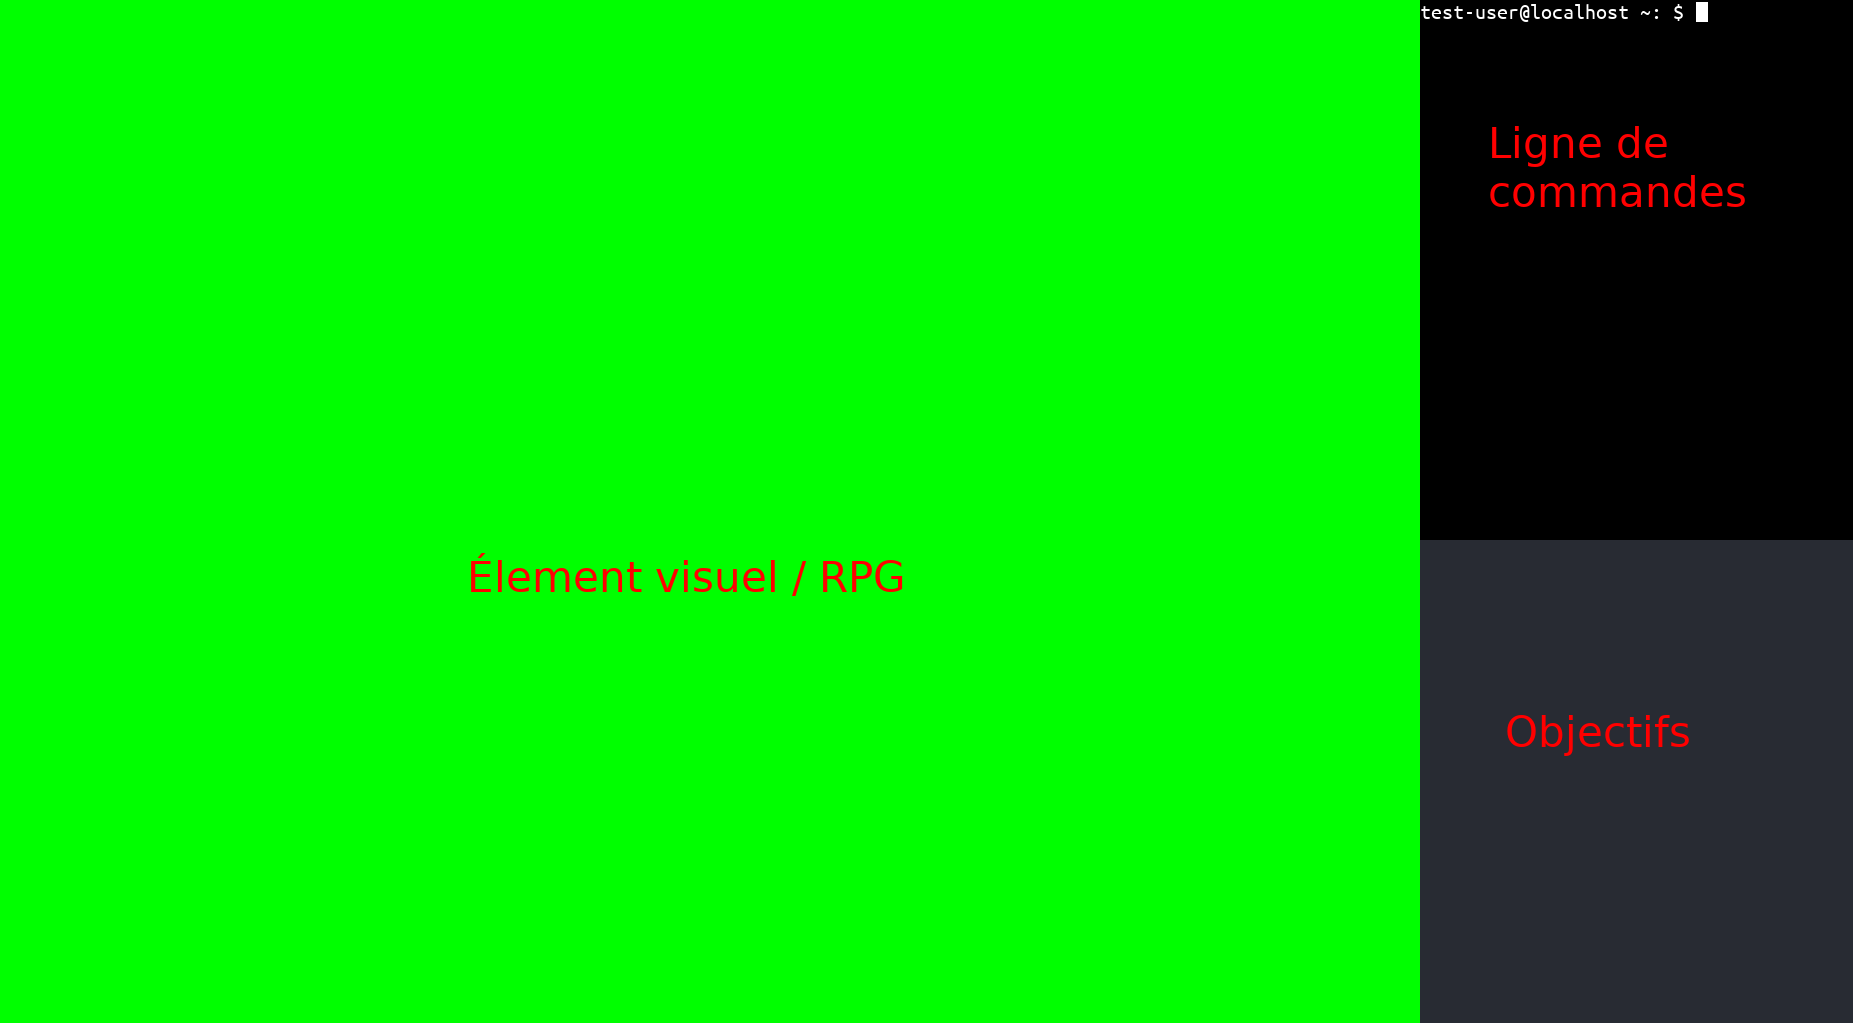
\includegraphics[width=\linewidth]{img/image1}
  \caption{Capture d'écran de la disposition par défault}
  \label{fig:screen1}
\end{figure}

\chapter{Analyse}
\section{Classes}
\subsection{game.mechanics.term.Term}
La classe \emph{Term} permet de créer des surfaces d'interaction tel que ligne de commande et entrée standard pour l’utilisateur, une fois initialisé elle charge la police de caractères monospace (en 22 pixels car c’est beaucoup plus lisible et agréable à utiliser), ensuite elle crée un dossier \emph{.shelladv} dans le dossier personnel de l’utilisateur (Exemple: \emph{/home/dalcjor/.shelladv} )
\subsection*{Attributs}

\begin{itemize}
  \item \mintinline{python}{surface : pygame.Surface}		$\rightarrow$ Surface principale du terminal
  \item \mintinline{python}{mono : pygame.font.Font}		$\rightarrow$ Police de caractère monospace
  \item \mintinline{python}{visualLine : List[str]}		$\rightarrow$ Lignes visibles sur la surface du terminal
  \item \mintinline{python}{lineRect : pygame.Rect}		$\rightarrow$ Rectangle de l’entrée utilisateur
  \item \mintinline{python}{blinkRect : pygame.Rect}		$\rightarrow$ Rectangle avec le rectangle clignotant
  \item \mintinline{python}{fontSurface : pygame.Rect}		$\rightarrow$ Rectangle avec les lignes précédentes
  \item \mintinline{python}{inInput : bool}			$\rightarrow$ Permet de savoir si l’utilisateur est en train d'entrer du texte
  \item \mintinline{python}{promptVisual: bool}			$\rightarrow$ Permet de savoir si le terminal doit afficher le prompt
  \item \mintinline{python}{bash: bool}				$\rightarrow$ Permet de savoir si le terminal doit exécuter les commandes entrées ou pas
  \item \mintinline{python}{currentTyping : str}		$\rightarrow$ Stock l’entrée utilisateur
  \item \mintinline{python}{blinkX : int}			$\rightarrow$ Position x du rectangle clignotant à côté du prompt
  \item \mintinline{python}{custom : str}			$\rightarrow$ Stock les prompts customisés
  \item \mintinline{python}{history : mechanics.term.History}	$\rightarrow$ Stock les prompts customisés
  \item \mintinline{python}{env : Dict[str, str]}		$\rightarrow$ Variables d'environnements semblables à celles présentes dans les systèmes UNIX
  \item \mintinline{python}{prompt: str}		$\rightarrow$ Permet de prendre connaissance du nom d’utilisateur, nom de la machine et le CWD (Current Work Directory)
  \item \mintinline{python}{tick: float}		$\rightarrow$ Heure actuel pour permettre de réguler la vitesse du blink (le rectangle à côté du prompt)

\end{itemize}

\end{document}
